\newday{09 April 2024}
	
	\action{PL information determination}
	
	\action{Given some set of data containing the inputs (eg mode coeffs or images) X and outputs (eg PL fluxes) y of a photonic lantern, quantify the amount of information preserved by the encoding, independent of any assumptions about the transfer function or reconstruction algorithm.}
	
	\action{First create files with the predictions from the models \filename{PSFRecontructorSuperBigFC70000-1} (for the original sized complex fields predictions) and \filename{CroppedBNFC70000-1} (for the cropped complex fields predictions). The predictions are made for the whole train dataset.}
	
	\action{\textbf{BRUTE FORCE ANALYSIS}:
		\begin{itemize}
			\item Pick 70000 random pair of frames
			\item Save euclidean distances for each of them
			\item Plot euclidean distances
			\item See if PSF similarity implies PL similarity
			\item Metric will be the ratio between PL output distances and PSF distances
			\item Perform ANOVA test for Uncropped, Cropped, PredictedUncropped, PredictedCropped pairs.
		\end{itemize}
	}
	
	\action{I compute the euclidean distances between pairs and store the pairs in \filename{pairsxx.npy} and \filename{euclidean\_distancesxx.npy}. The \filename{euclidean\_distancesxx.npy} array has shape of 1000x5, each column being the distance between pairs of psf fluxes, original complex fields, cropped complex fields, predicted complex fields and predicted cropped complex fields.}
	
	\action{The complex fields are 2x128x128 and the cropped complex fields are 2x64x64, when I say predicted I mean the complex generated by the models.	}
	
	\rule{0.5\textwidth}{0.5pt}\\

	{\large \textbf{EXPERIMENT Euclidean distances}}\\
	
	\begin{figure*}[ht!]
		\centering
		\subfloat[Train subset 0]{%
		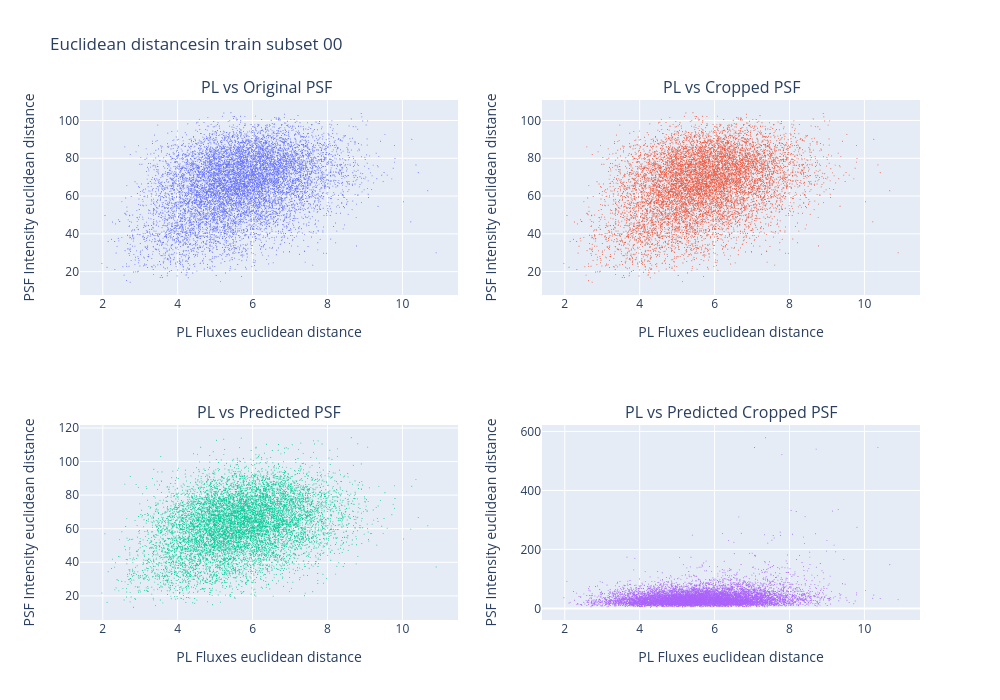
\includegraphics[width=0.45\textwidth]{euclideans_00.png}}
		\subfloat[Train subset 1]{%
		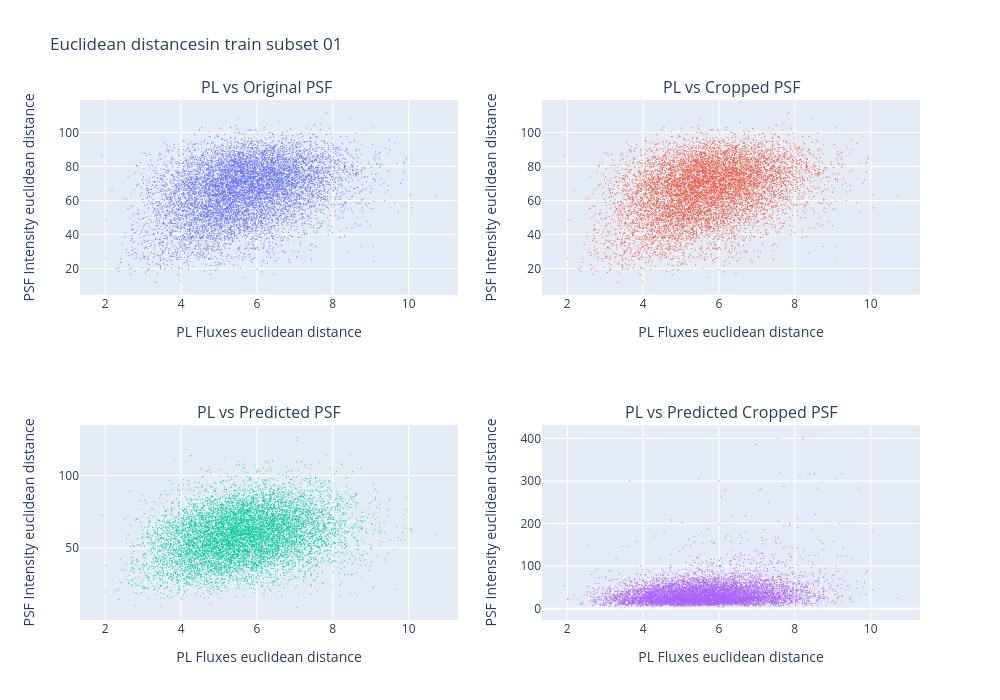
\includegraphics[width=0.45\textwidth]{euclideans_01.png}}\\
		\subfloat[Train subset 2]{%
		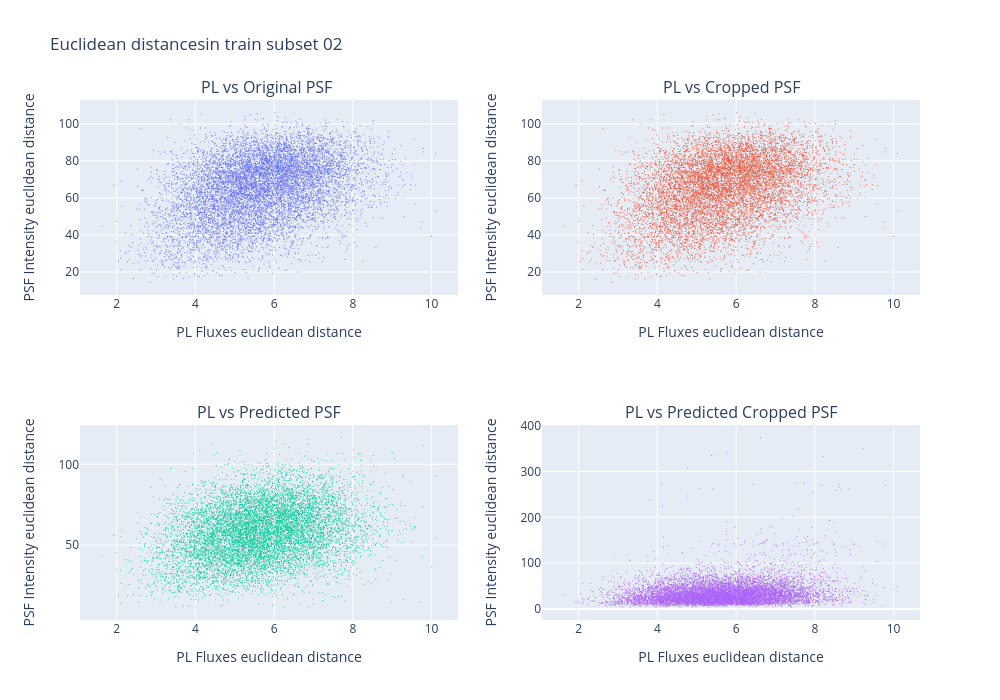
\includegraphics[width=0.45\textwidth]{euclideans_02.png}}
		\subfloat[Train subset 3]{%
		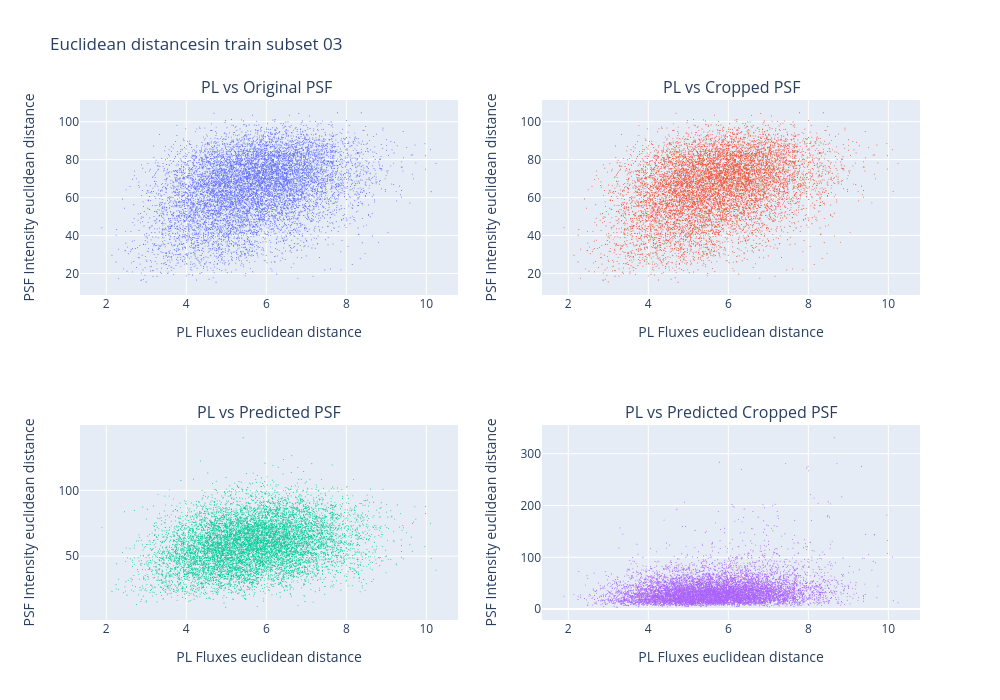
\includegraphics[width=0.45\textwidth]{euclideans_03.png}}\\
		\subfloat[Train subset 4]{%
		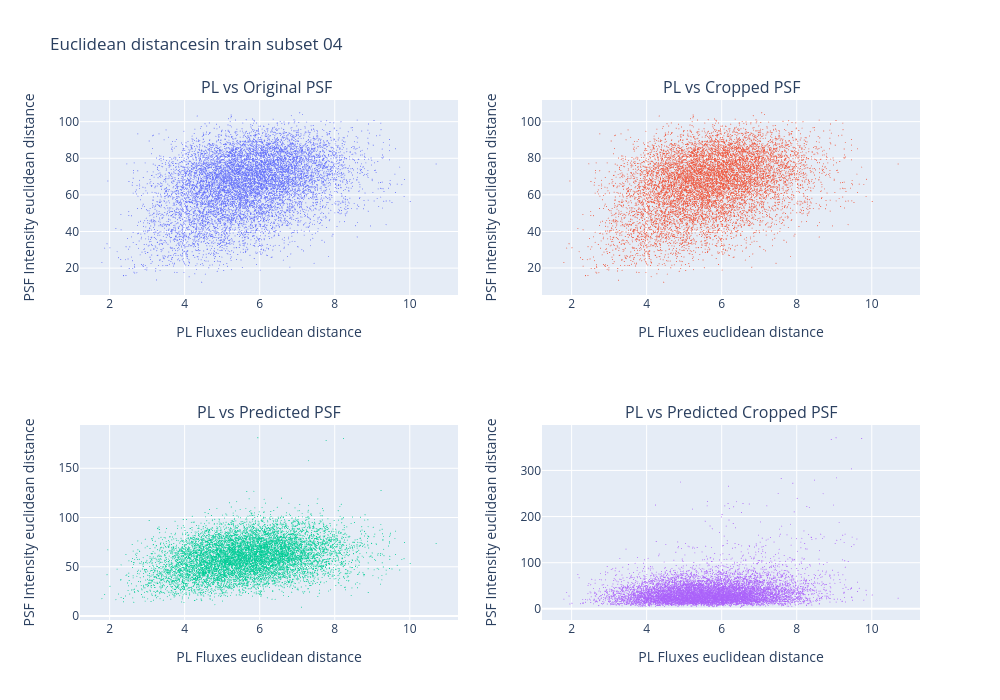
\includegraphics[width=0.45\textwidth]{euclideans_04.png}}
		\subfloat[Train subset 5]{%
		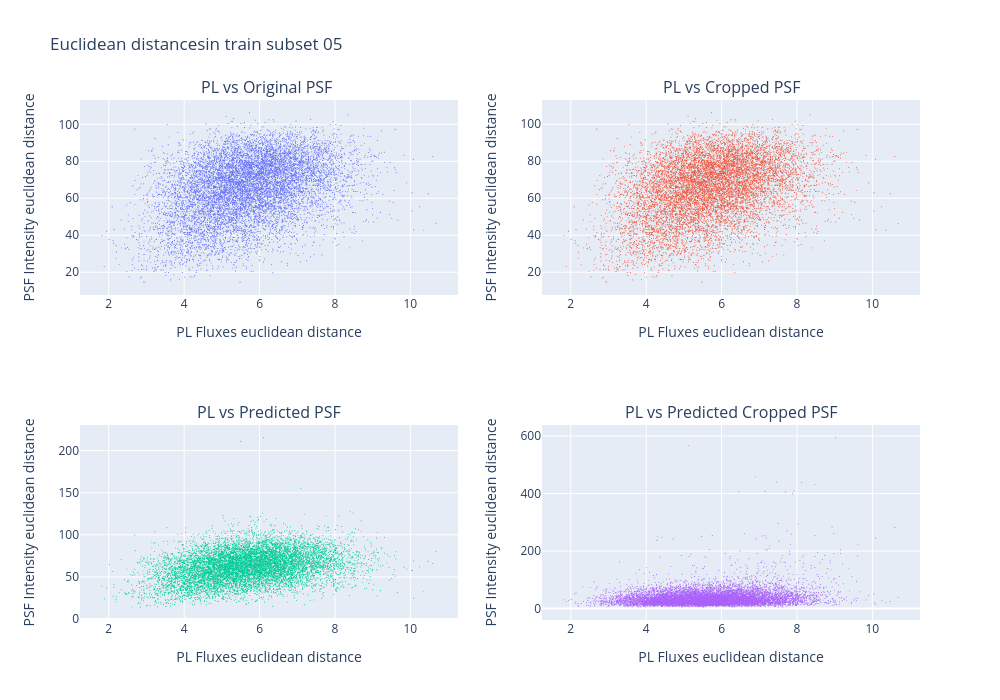
\includegraphics[width=0.45\textwidth]{euclideans_05.png}}\\
		\subfloat[Train subset 6]{%
		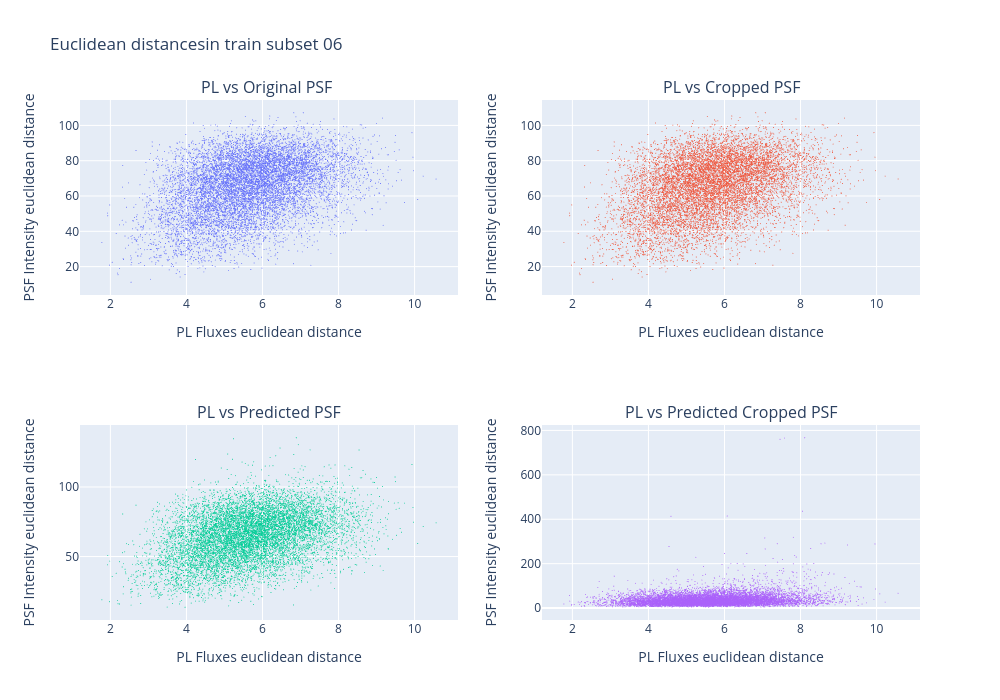
\includegraphics[width=0.45\textwidth]{euclideans_06.png}}
		\caption{Euclidean distances between PL and PSF pairs}\hspace{\fill}
	\end{figure*}
	
\FloatBarrier	
\rule{0.5\textwidth}{0.5pt}\\
	
\finishday